\chapter{Conceptual Model}\label{ch:conceptual}

In this chapter, we propose a conceptual model named \frappe{}~\cite{DBLP:conf/semweb/BalduiniV15}. \frappe{} is a vocabulary that bridge the gap between the data engineer and visual interface designers for enabling visual analytics for the detection, the understanding and the interpretation of spatio-temporal data.
We introduce the problem, solved by \frappe{}, in Section~\ref{sec:conc-intro}.
In Section~\ref{sec:conc-fr-1}, we present an overview of the first version of \frappe{}.
In Section~\ref{sec:conc-fr-2}, we propose \frappe{} 2.0, an extension of the original vocabulary where we expand the provenance fragment and add a content related fragment.
Finally, Section~\ref{sec:conc-fr-2-analysis} presents an overview of the analysis enabled by \frappe{} 2.0.

\section{Introduction and Problem Statement}\label{sec:conc-intro}
Since the last decade, the rapid increase of sources, which expose geo-located time-varying data, has been drawing attention of those who are looking for data-driven decision making. 
The availability of social media, telecommunication, traffic and weather data improved the ability to capture peoples' interests, habits and preferences.

In particular, the growing availability of urban data sources (see Chapter~\ref{ch:uda}) stimulated the research of a holistic conceptual model to manage data variety in a comprehensive way. The current interest is for solutions that enable the fusion of streaming heterogeneous data to enable reactive decisions.

One of the main assumptions of any smart-city approach is to work upon a layer of data collected from the city itself that describes its dynamics. The city evolution can span multiple layers, from architecture to urban design, from population composition and migrations to citizen behaviors and interests. Each of these layers has a different dynamics and speed of change.
Therefore, it should be monitored collecting data from different sources and using multiple analysis techniques (see Section~\ref{sec:uda-analysis}). 

\begin{figure}[t]
\centering
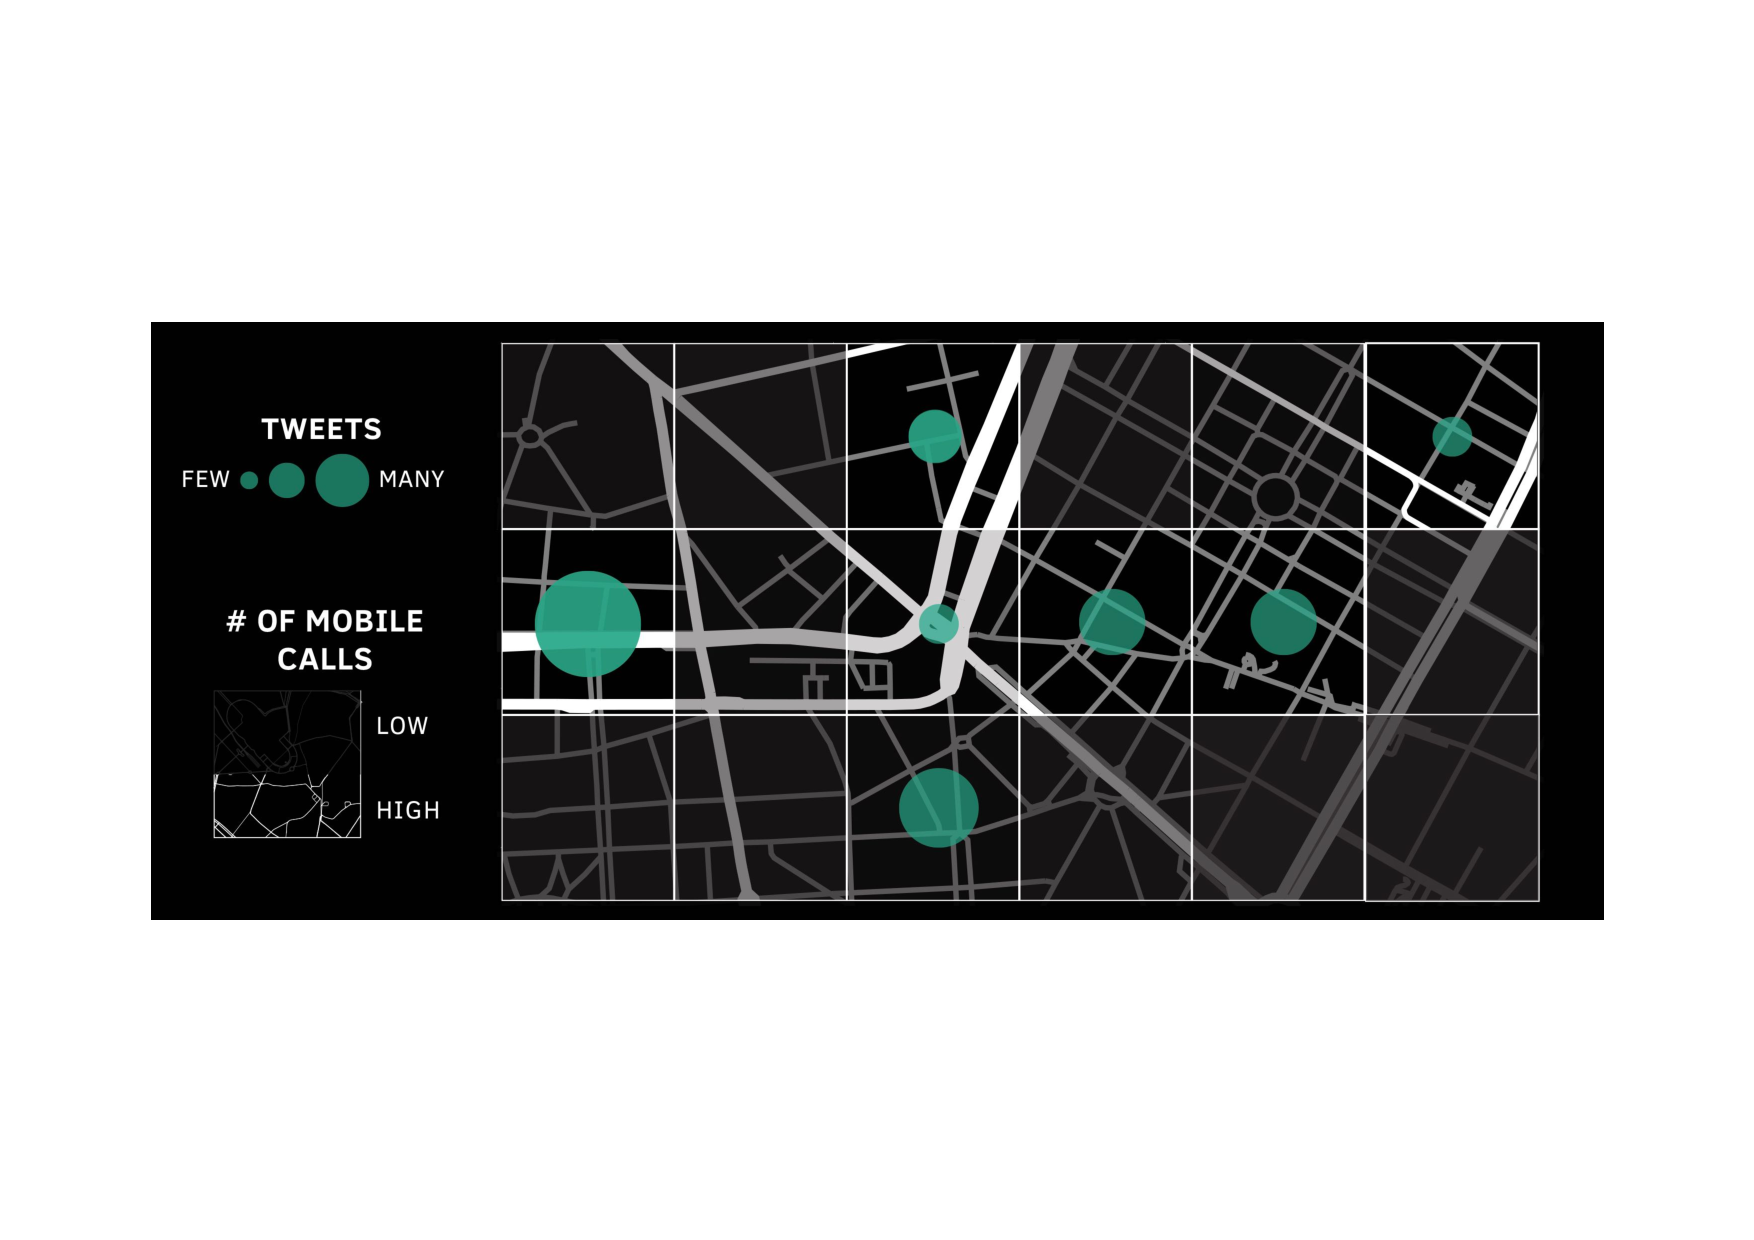
\includegraphics[width=0.8\textwidth]{img/real-world-rep}
\caption{A real-world example of visual analytics of two heterogeneous datasets. (source~\cite{DBLP:conf/semweb/BalduiniV15}).}
\label{fig:real-world-rep}
\end{figure} 

In particular, our research question, presented in Section~\ref{sec:prob_rq}, refers to visual analytics\footnote{The science of analytical reasoning facilitated by interactive visual interfaces~\cite{cook2005illuminating}.} as a way for making sense of heterogeneous spatio-temporal streaming data.
For instance, Figure~\ref{fig:real-world-rep} illustrates a real case of visual analytics for a general audience we experimented during the Milano Design Week events (see Section~\ref{sec:cs-mdw-2014}).
The Figure presents a grid of 6x3 cells overlaid to a city street map. Green circles can appear in each cell. They visually represent the number of tweets posted in a time interval from each cell. The fill color opacity value of each cell is, instead, mapped to the number of mobile calls from each cell. As we showed in Section~\ref{sec:cs-mdw-2014}, people without specific expertise in data analytics can easily guess the cells where the two signals are correlated.

Unfortunately, data is not often ready for visual analytics.
A gap exists between the terms used by the designers who create the visual analytics interface and those used by the computer scientists who prepare the data. The designers expect data aggregated over time and space, while the data engineers talk about fine-grained geo-located time-varying data.
For instance, in 2012, during the BOTTARI experiment (see Section~\ref{sec:uda-bottari}) in the city of Seoul, we model data using SMA ontology (see Figure~\ref{fig:sma-onto}).
SMA extends the SIOC vocabulary\footnote{\url{http://sioc-project.org/}} adding the spatial aspect. To do so, it exploits terms from W3C WGS-84 vocabulary\footnote{\url{https://www.w3.org/2003/01/geo/}}.
SMA poses the attention only on the raw data representation.
It does not include any specific concept to represent data aggregations or data abstractions to enable advanced analytics, which is one of the goal of this thesis.

\begin{figure}[t]
\centering
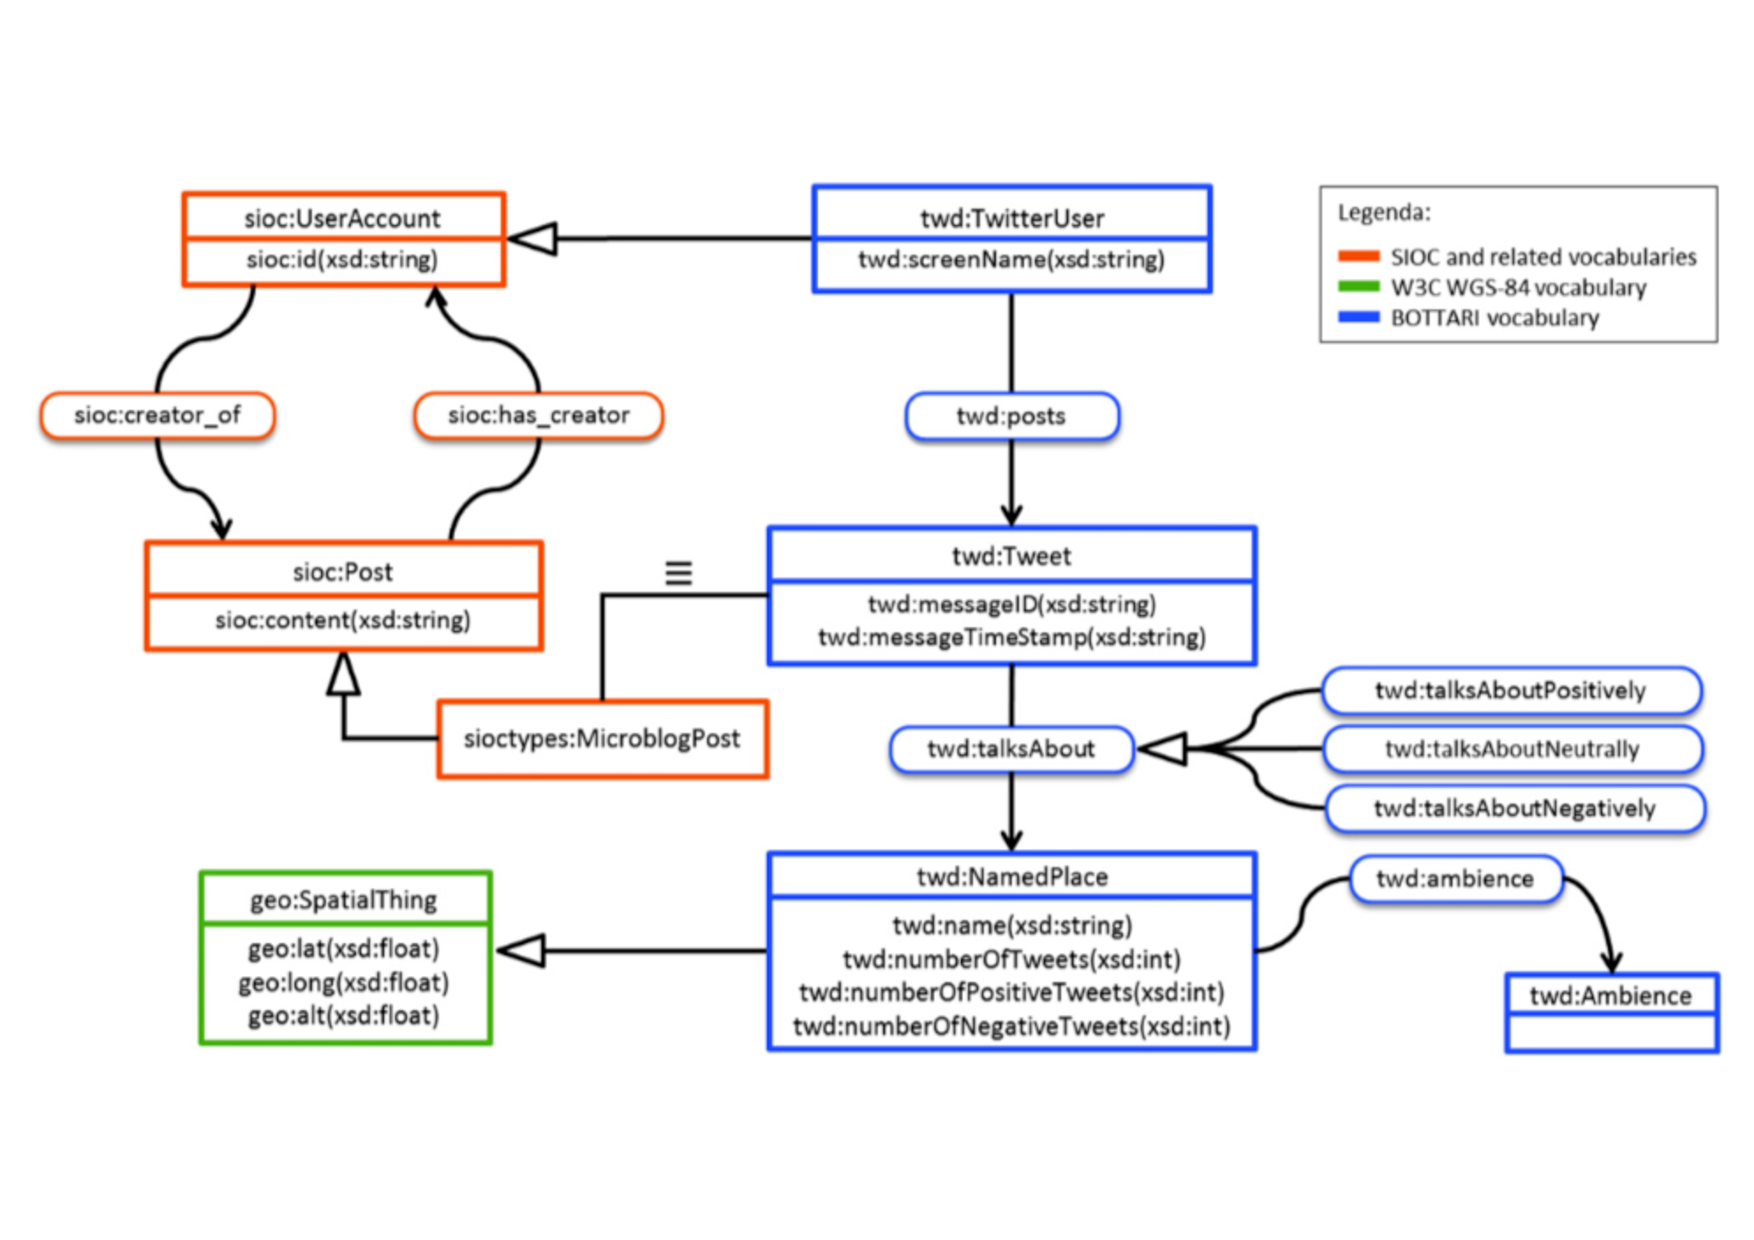
\includegraphics[width=0.85\textwidth]{img/sma-ontology}
\caption{Overview of the SMA ontology used in the BOTTARI project to model the data (source \cite{DBLP:journals/ws/BalduiniCDVHLKT12}).}
\label{fig:sma-onto}
\end{figure}

During years of collaboration with the Design Department of Politecnico di Milano\footnote{\url{https://densitydesign.org/}}, we discover that image processing terms like \textsf{Pixel} or \textsf{Frame} are common among both designers and data engineers. They represent a bridge between who prepare the data and who create the interfaces for visualizing it.

With this observation in mind, in order to answer the research questions, we formulated the hypotheses \textsf{Hp.1.1} and \textsf{Hp.1.2}

\begin{itemize}[leftmargin=42pt]
\item[\textsf{Hp.1.1}] A conceptual model containing terms from the image processing domain can represent spatio-temporal data in an extendable and coherent way with a minimal encoding bias and a minimal ontological commitment.
\item[\textsf{Hp.1.2}] Visual analytics interfaces built directly on data represented with the conceptual model of Hp.1.1 are guessable\footnote{The guessability is defined as the measure of the cost to the user involved in using an interface to perform a new task for the first time. The lower the cost, the higher the guessability~\cite{moyes1993icon}. The cost can be measured in terms of time, errors, or effort.}.
\end{itemize}

\section{\frappe{} 1.0}\label{sec:conc-fr-1}
In this section, we propose our first attempt to create a conceptual model to represent spatio-temporal data.
Section~\ref{sec:conc-fr-1-mod} exposes the main concepts behind \frappe{} and the development methodology.
In Section~\ref{sec:conc-fr-1-eval}, we present an evaluation of \frappe{} 1.0 based on its adherence to the Tom Gruber's  principles~\cite{DBLP:journals/ijmms/Gruber95}.
Finally, Section~\ref{sec:conc-fr-1-synth-ex} presents a working example, where we use \frappe{} 1.0 to model the data of the DEBS Grand Challenge 2015\footnote{\url{http://www.debs2015.org/call-grand-challenge.html}}.

\subsection{The Conceptual Model}\label{sec:conc-fr-1-mod}
In order to verify the hypotheses \textsf{Hp.1.1} and \textsf{Hp.1.2}, we proposed the conceptual model \frappe{}. It is named out of its four main concepts: Frame, Pixel, Place and Event.
In this section, we refer to \frappe{} 1.0 as \frappe{}.

\begin{figure}[t]
\centering
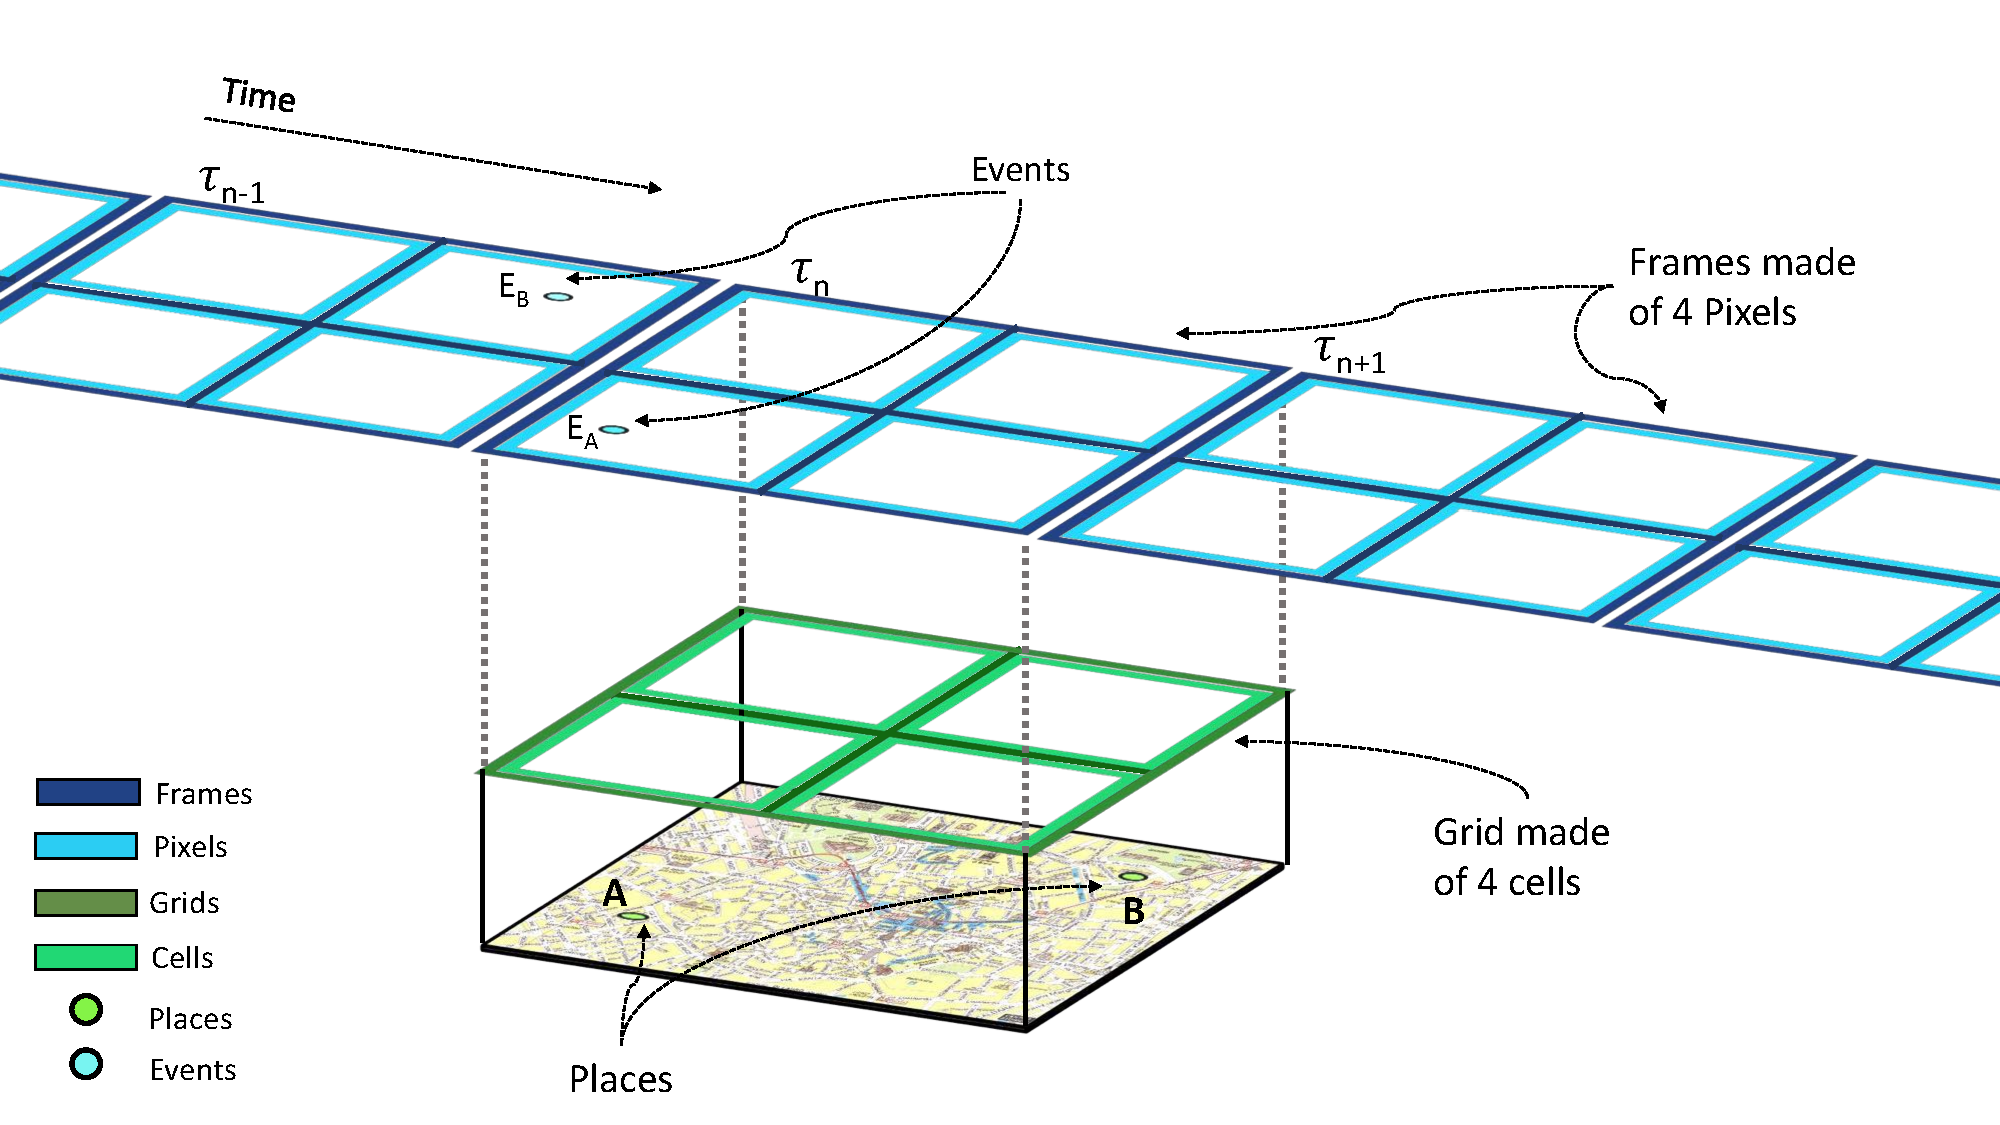
\includegraphics[width=0.8\textwidth]{img/conceptual-model-overview}
\caption{A high-level view of \frappe{} including 3 \textsf{Frame}s made of
4 \textsf{Pixel}s containing the \textsf{Place}s where the \textsf{Event}s happen.}
\label{fig:overview}
\end{figure}

\frappe{} ontology is formalized using the version 2 of the Web Ontology Language (see Section~\ref{sec:owl}). It reuses GeoSparql~\cite{battle2011geosparql} as geographical data model, the Time~\cite{Hobbs2006} and Event ontologies~\cite{RaimondAbdallahEventOntology2007}) as time/event vocabularies, and PROV-~O~\cite{w3c-prov-o} as provenance ontology. 

\frappe{} enables an OBDA approach for the data analysis by exploiting the terms imported from GeoSparql, Time, Event and PROV-O ontologies without any axiomatization. This is because OBDA requires OWL2-QL ontologies, while \frappe{} with the imported ontologies is in OWL2 Full. 

\frappe{} offers a high level view of the detection, the understanding, and the interpretation of geo-spatial time-varying data.
It uses a digital image processing metaphor (see Figure \ref{fig:overview}) to track the three main dimensions of analysis introduced in Section~\ref{sec:uda-analysis}: space, time, and content. 

\frappe{} assumes that the real world can be described as a bi-dimensional space, where \textsf{Event}s happen in \textsf{Place}s over time. For instance, a user making a check-in on a geo-located social network generates an event in a place. A taxi ride generates a sequence of two events (a pick-up and a drop-off) in two distinct places. A garbage collector truck generates a sequence of events around the city in different points in time, one for each trash bin it cleans up.

\begin{figure}[t]
\centering
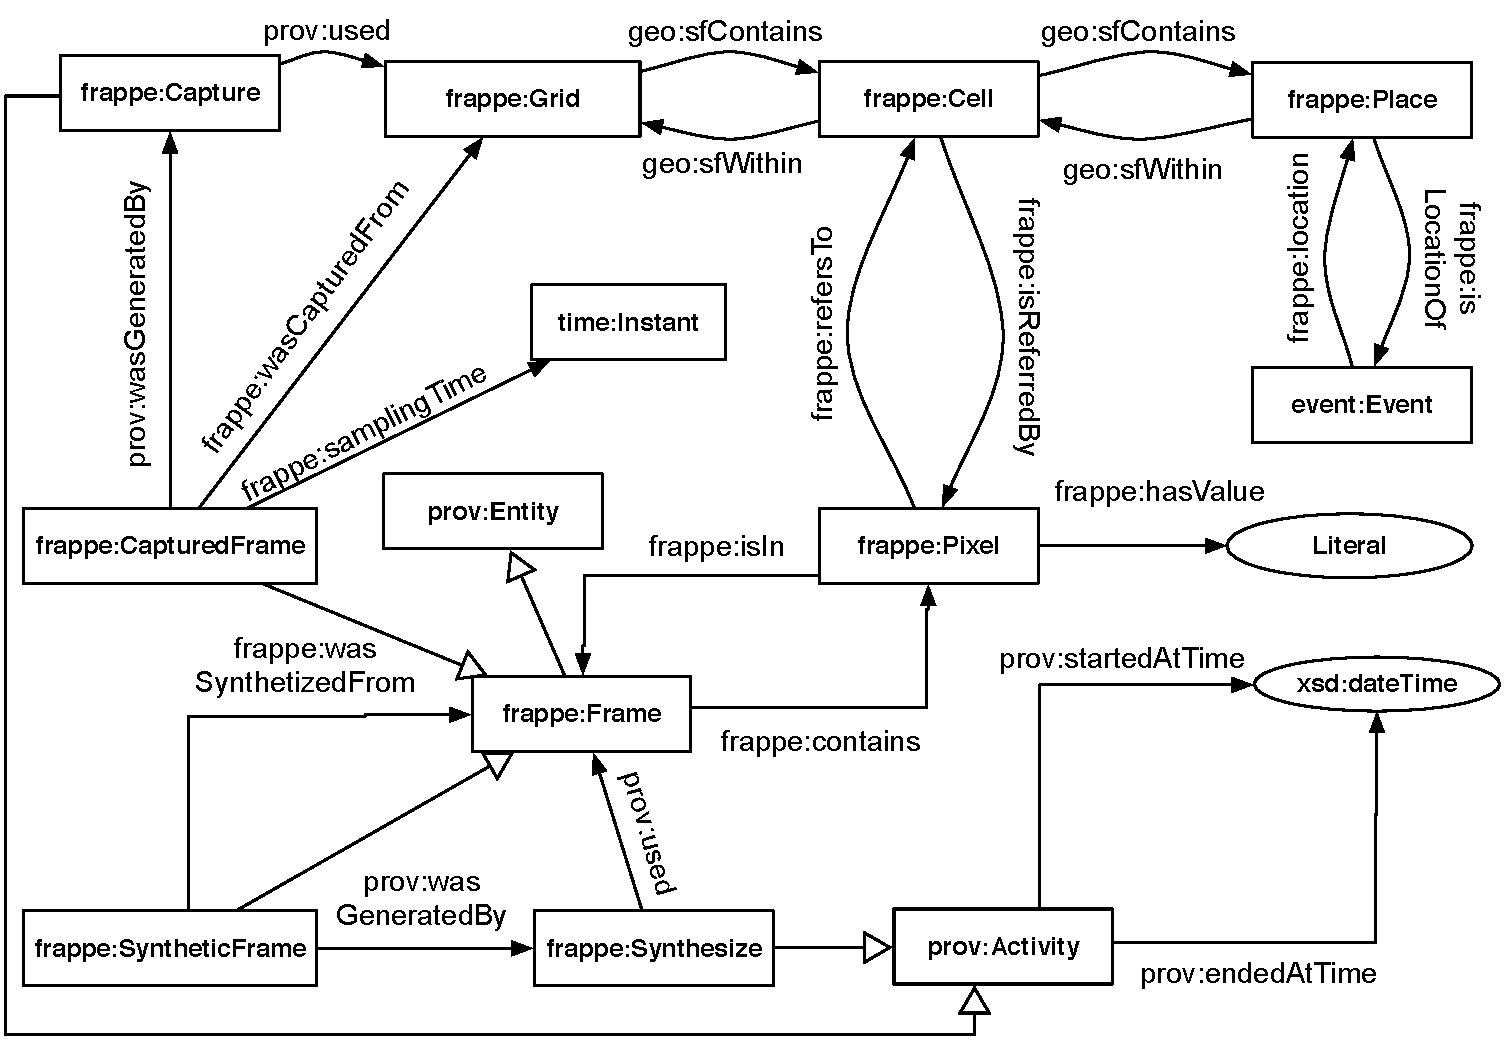
\includegraphics[width=0.85\textwidth]{img/conceptual-model-original-core}
\caption{The UML representation of the original version of the \frappe{} ontology}
\label{fig:original-core}
\end{figure} 

Figure~\ref{fig:original-core} depicts all the main concepts in the model.
\frappe{} is organized in three interconnected parts: the geographical, the time-varying and the provenance fragments.
It proposes to capture the digital footprints of what happens in the real-world as a sequence of \textsf{Frame}s. A \textsf{Grid} sits between the physical world and the frames of the film. It decomposes the physical world in \textsf{Cell}s. Each frame is, therefore, decomposed accordingly in \textsf{Pixel}s.

More formally, \textsf{Place}, \textsf{Cell} and \textsf{Grid} belong to the geographical fragment and reuse terms from the GeoSparql vocabulary~\cite{battle2011geosparql}. 
%They are geosparql \texttt{Feature}s whose default geometry are respectively a \texttt{point}, a \texttt{surface} and a \texttt{multisurface}. 
\textsf{Event}, \textsf{Pixel} and \textsf{Frame} are in the time-varying part. The \textsf{Event} term is borrowed from the Event ontology~\cite{RaimondAbdallahEventOntology2007}. 
The provenance part includes the activities \textsf{Capture} and \textsf{Synthesize} and reuses the PROV Ontology~\cite{w3c-prov-o} (PROV-O).

An \textsf{Event} has a \textsf{location} in a \textsf{Place} in a \textsf{Cell} -- the basic spatial unit of aggregation of information in \frappe{} -- which, in turn, is in a \textsf{Grid}.

A \textsf{Pixel} is the time-varying representation of a \textsf{Cell}. It is the only element in \frappe{} 1.0 that carries information through the \textsf{hasValue} data property. As in image processing, this value represents a measure of intensity of some phenomenon in the real world. For instance, it can represent the number of micro-posts posted in a given time interval in a certain \textsf{Cell}. Each \textsf{Pixel} \textsf{refersTo} a single \textsf{Cell}, contrariwise a \textsf{Cell} could be \textsf{referredBy} many different \textsf{Pixel}s that captures different information associated to the same \textsf{Cell}, e.g., the already mentioned number of micro-posts, but also the number of mobile phone calls or the number of goods' pick-ups.

Similarly, a \textsf{Frame} is the time-varying counterpart of a \textsf{Grid} and a sequence of \textsf{Frame}s composes the film of the evolution of a physical portion of the world over time. 
\frappe{} distinguishes between two specializations of \textsf{Frame}s: the \textsf{CapturedFrame}s and the \textsf{SyntheticFrame}s. 
\textsf{Frame} and \textsf{Grid} are \textit{Entity} in PROV-O. This is because \frappe{} proposes the ternary relationships \textsf{Capture} and \textsf{Synthesize} as specializations of the relationship \textit{Activity} of PROV-O.

A \textsf{CapturedFrame} \textit{wasGeneratedBy} a \textsf{Capture} \textit{Activity} \textit{startedAtTime} $\tau_i$ and \textit{endedAtTime} $\tau_j$ that \textit{used} a given \textsf{Grid}. It \textsf{contains} a \textsf{Pixel} for every \textsf{Cell} in the \textsf{Grid} it \textsf{wasCapturedFrom}. Different \textsf{Frame}s represent different images of the observed phenomena at the same \textsf{samplingTime} (e.g., a frame captured the volume of the social activity while another one captured the volume of the mobile phone calls at 12.00).
The object property \textsf{wasCapturedFrom} is the result of the chaining of the two \textit{wasGeneratedBy} and \textit{used} object properties. Moreover, the value of the \textsf{samplingTime} data property, which describes the \textsf{CapturedFrame}, is the one assigned to the \textit{startedAtTime} data property that describes the captured activity. 

Similarly, a \textsf{SyntheticFrame} \textit{wasGeneratedBy} by a \textsf{Synthesize} \textit{Activity} that \textit{used} one or more \textsf{Frame}s. The idea is to derive a \textsf{Frame} from one or more others. The \textsf{Synthesize} operation can be a filter applied to the values of the pixels, or an aggregation of values of \textsf{Pixel}s across \textsf{Frame}s or the difference between the values associated to the \textsf{Pixel}s of two different \textsf{Frame}s. 

We develop \frappe{} using METHONTOLOGY~\cite{fernandez1997methontology} (see Section~\ref{sec:onto-eng}) methodology by following the whole ontology life cycle.
%specification
We started from the specification phase following, in the scoping activity, a middle-out approach (see Section~4.1 in~\cite{fernandez1997methontology}). We exploited terms from image processing and spatial glossaries in order to find the primary concepts of \frappe{} and to verify, at the earliest possible stage, the conciseness and completeness of our specification. 
%conceptualization
We then conceptualized the specification and produced a complete  Glossary of Terms (GT).
%integration
Most of the concepts in \frappe{} are directly integrated from other domain specific ontologies (e.g., Instant from Time ontology~\cite{Hobbs2006}, Activity from PROV-O ontology~\cite{w3c-prov-o}, etc.)
%Evaluation

\subsection{Adherence to the Tom Gruber's Principles} \label{sec:conc-fr-1-eval}
We evaluated \frappe{}, by checking if it adhere the five principles of Tom Gruber~\cite{DBLP:journals/ijmms/Gruber95}: 
clarity, coherence, minimal encoding bias, minimal ontological commitment and extendibility.

\frappe{} satisfies the \textit{clarity} principle because all definitions are documented in natural language (see the version of \frappe{} published on github\footnote{\url{https://github.com/streamreasoning/FraPPE.git}}). The terms proposed in \frappe{} are: (i) common terms in spatial-related vocabularies (e.g., \textsf{Place}, \textsf{Cell}, \textsf{Grid}); (ii) well known terms of the image processing domain (e.g., \textsf{Pixel}, \textsf{Frame}, \textsf{Capture}, or \textsf{Synthesize}); and (iii) terms defined in other ontologies (e.g., Event, Instant, Entity, or Activity). 

\frappe{} has a \textit{minimal encoding bias} because it is encoded in OWL2. Moreover, we explicitly avoided adding cardinality restrictions, because, in our works (see Chapter~\ref{ch:case-studies}), we use \frappe{} to integrate data following an Ontology-Based Data Access approach which requires OWL2 profile that does not include cardinality restrictions.   

\frappe{} requires a \textit{minimal ontological commitment}, meaning that, as Tom Gruber recommended, \frappe{} makes as few claims as possible about the geo-located time-varying data being modeled allowing who uses \frappe{} to specialize and instantiate it as needed.

We tested in details that \frappe{} is \textit{extendable} by successfully modeling the dataset made available by ACM DEBS 2015 Grand Challenge\footnote{\url{http://www.debs2015.org/call-grand-challenge.html}}, for all the details, see Section~\ref{sec:conc-fr-1-synth-ex}.
Moreover, we check the extendibility of \frappe{} while using it in the experiences reported in the Chapter~\ref{ch:case-studies}. For further details see Section~\ref{sec:cs-conclusion}.

Last but not least, \frappe{} is \textit{coherent}, i.e., all \frappe{} inferences at T-box level are consistent with the definitions and in modeling A-boxes containing social, telecommunication, environment, traffic, and energy consumption data, we never inferred inconsistent or meaningless data.

\begin{figure}[p]
\begin{minipage}{0.95\linewidth}
\begin{lstlisting}[label={lst:debs}, caption={Fraction of the model representing ACM DEBS Grand Challenge 2015 Data}, style=N3]
@prefix frGrid: <http://streamreasoning.org/debsGC/Grids/> .
@prefix frCell: <http://streamreasoning.org/debsGC/Cells/> .
@prefix frPixel: <http://streamreasoning.org/debsGC/Pixels/> .
@prefix frPlace: http://streamreasoning.org/debsGC/Places/:> .
@prefix frEvent: <http://streamreasoning.org/debsGC/Events/> .
@prefix frFrame: <http://streamreasoning.org/debsGC/Frames/> .
@prefix frCapture: <http://streamreasoning.org/debsGC/Captures/> .

frGrid:Grid_1 gs:sfContains frCell:Cell_1, frCell:Cell_2 .

frCell:Cell_1 a fr:Cell ;
    rdfs:label "39460"^^xsd:long ;
    fr:isReferredBy frPixel:1356995100000_39460 ;
    gs:sfContains frPlace:A ;
    gs:sfWithin frGrid:Grid_1 .

frPlace:A a sf:Point ;
    fr:isLocationOf frEvent:E_B ;
    gs:asWKT "POINT( 40.715008 -73.96244 )"^^gs:wktLiteral ;
    gs:sfWithin frCell:Cell_1 .

frEvent:E_A a fr4d:PickUpEvent ; 
    a event:Event ;
    event:time [ a time:Instant ; 
       time:inXSDDateTime "2013-01-01T00:00:00"^^xsd:dateTime ] ;
    fr:location frPlace:A> ;
    fr4d:hackLicense "E7750A37CAB07D0DFF0AF7E3573AC141"^^xsd:string ;
    fr4d:medallion "07290D3599E7A0D62097A346EFCC1FB5"^^xsd:string .

frEvent:E_B a fr4d:DropOffEvent ; 
    a event:Event ;
    event:time [ a time:Instant ; 
       time:inXSDDateTime "2013-01-01T00:02:00"^^xsd:dateTime ] ;
    fr:location frPlace:B ;
    fr4d:connected frEvent:E_A ;
    fr4d:fareAmount "3.5"^^xsd:double ;
    fr4d:mtaTax "5.0"^^xsd:double ;
    fr4d:paymentType "CSH"^^xsd:string ;
    fr4d:surcharge "5.0"^^xsd:double ;
    fr4d:totalAmount "4.5"^^xsd:double ;
    fr4d:tripDistance "0.44"^^xsd:long ;
    fr4d:tripTime "120"^^xsd:long .

frPixel:1356995100000_39460 a fr:Pixel ;
    fr:isIn frFrame:1356995100000 ;
    fr:refers frCell:Cell_1 .

frFrame:1356995100000 a fr:CapturedFrame ;
    fr:contains frPixel:1356995100000_39460, 
    frPixel:1356995100000_39461 ;
    fr:samplingTime [ a time:Instant ; 
       time:inXSDDateTime "2013-01-01T00:05:00"^^xsd:dateTime ];
    fr:wasCapturedFrom frGrid:Grid_1 ;
    prov:wasGeneratedBy frCapture:1356995100000 .
\end{lstlisting}
\end{minipage}
\end{figure} 

\subsection{Working Example} \label{sec:conc-fr-1-synth-ex}

\begin{figure}[t]
\begin{minipage}[t]{0.95\linewidth}
\begin{lstlisting}[label={lst:sparql-debs}, caption={Sparql query to create the \textsc{SytheticFrame}s containing the \textsc{Pixel}s with the profitability value.}, style=SPARQL]
PREFIX   rdf:<http://www.w3.org/1999/02/22-rdf-syntax-ns#>
PREFIX   xsd:<http://www.w3.org/2001/XMLSchema#>
PREFIX   time:<http://www.w3.org/2006/time#>
PREFIX   f4d:<http://streamreasoning.org/ontologies/frappe4debs#>
PREFIX   prov:<http://www.w3.org/ns/prov#> 
PREFIX   event:<http://purl.org/NET/c4dm/event.owl#>
PREFIX   geos:<http://www.opengis.net/ont/geosparql#>
PREFIX   rdfs:<http://www.w3.org/2000/01/rdf-schema#>
PREFIX   fr:<http://streamreasoning.org/ontologies/frappe#>
PREFIX   sf:<http://www.opengis.net/ont/sf#>

CONSTRUCT{
    concat("frFrame:",now()") a fr:SyntheticFrame ;
    fr:contains ?pixel ;
    fr:samplingTime [ a time:Instant ; 
    		time:inXSDDateTime ?time ] ;
    fr:wasSynthesizedFrom ?frame . 
    ...
}
WHERE {
	?pixel f:isIn ?frame ;
	fr:refers ?cell .
	?cell geos:sfContains ?place ;
	rdfs:label ?cellLabel .
	?place f:isLocationOf ?e .
	?e a f4d:DropOffEvent ;
	f4d:totalAmount ?t .
	?frame time:hasBeginning ?beginning .
	?beginning time:inXSDDateTime ?time .
	FILTER(?time >= \"2013-01-01T00:10:00\"^^xsd:dateTime
    && ?time <= \"2013-01-01T00:15:00\"^^xsd:dateTime)"
}
GROUP BY ?pixel ?cell ?cellLabel
\end{lstlisting}
\end{minipage}
\end{figure} 

The ACM DEBS 2015 Grand Challenge proposes a taxi route analysis scenario based on a grid of 150x150 Kms with cells of 500x500 m. A stream of data represents the route of a taxi rides in terms of: (i) taxi description, (ii) pick-up and drop-off information (e.g., geographical coordinates of the place and time of the event), and (iii) ride information (e.g., tip, payment type and total amount).
In Listing~\ref{lst:debs}, we report a subset of the information representing a single taxi ride in \frappe{}. The pick-up \textsf{Event} represents the start of the ride and contains the taxi id. The drop-off \textsf{Event} represents the end of the trip and it is connected to all the information about the ride. The fragment models the geographical part of the ride using two \textsf{Place}s within two different \textsf{Cell}s of a single \textsf{Grid}. Moreover, it models the time varying-part of the ride using two \textsf{Event}s captured in two \textsf{Pixel}s of a single \textsf{Frame} along with the provenance part through the \textsf{Capture} activity. Indeed, we use all \frappe{} concepts, we specialize \textsf{Event} in \textsf{PickUpEvent} and \textsf{DropOffEvent}, and we extend the vocabulary adding two attributes (e.g., \textsf{tripTime}, and \textsf{totalAmount}) and an object property (i.e., \textsf{connected}) specific of the taxi ride domain.

\begin{figure}[t]
\begin{minipage}{0.95\linewidth}
\begin{lstlisting}[label={lst:synthetic-debs}, caption={Fragment of the model that represents a \textsc{SytheticFrame}}, style=N3]
frFrame:1356995700000 a fr:SyntheticFrame ;
    fr:contains frPixel:1356995700000_39462, 
    frPixel:1356995700000_39463 ;
    fr:samplingTime [ a time:Instant ; 
    		time:inXSDDateTime "2013-01-01T00:15:00"^^xsd:dateTime ];
    prov:wasGeneratedBy frSynthesize:1356995700000 ;
    fr:wasSynthesizedFrom frFrame:1356994800000, 
    		frFrame:1356995100000, 
            frFrame:1356995400000, 
            frFrame:1356995700000. 

frSynthesize:1356995700000 a prov:Activity ;
	prov:startedAtTime "2013-01-01T00:15:00"^^xsd:dateTime .

frPixel:1356995700000_39462 a fr:Pixel;
    fr:isIn frFrame:1356995700000 ;
    fr:refers frCell:Cell_1 ;
    fr:hasValue "37"^^xsd:integer.

frPixel:1356995700000_39463 a fr:Pixel ;
    fr:isIn frFrame:1356995700000 ;
    fr:refers frCell : Cell_2 ;
    fr:hasValue "65"^^xsd:integer.
\end{lstlisting}
\end{minipage}
\end{figure} 

Synthetic frames are also important in representing the data of the challenge. One of the problems, assigned to the challengers, asks to compute the top profitable cells for a given time interval. Listing~\ref{lst:synthetic-debs} contains the representation of the \textsf{SytheticFrame}, named \textsf{frFrame:1356995700000}, computed by the \textsf{Synthesize} activity (\textsf{frSynthesize:1356995700000}) represented by the SPARQL query presented in Listing~\ref{lst:sparql-debs}. The \textsf{SyntheticFrame}, \textsf{wasSynthesizedFrom} four different \textsf{CapturedFrame}s, and contains two \textsf{Pixel}s, associated to two different \textsf{Cell}s with different values of profitability (number of \textsf{DropOffEvent}).

\section{\frappe{} 2.0} \label{sec:conc-fr-2}
In order to extend the expressiveness of \frappe{} and enable more advanced analysis (see Section~\ref{sec:conc-fr-2-analysis}), we propose \frappe{} 2.0.
We, mainly, extended the original \frappe{} by improving the provenance fragment, in order to specialize the \textsf{Agent} concept, and by adding the content related fragment, in order to enable more fine grained analysis. 

Figure~\ref{fig:extended-core} depicts a UML representation of the \frappe{} 2.0 model, only the extended parts is presented in the figure.
As highlighted by different colors, \frappe{} 2.0 is organized in different interconnected parts: the white one is related to time, the light gray one to content, and the dark gray one to provenance. 

\begin{figure}[t]
\centering
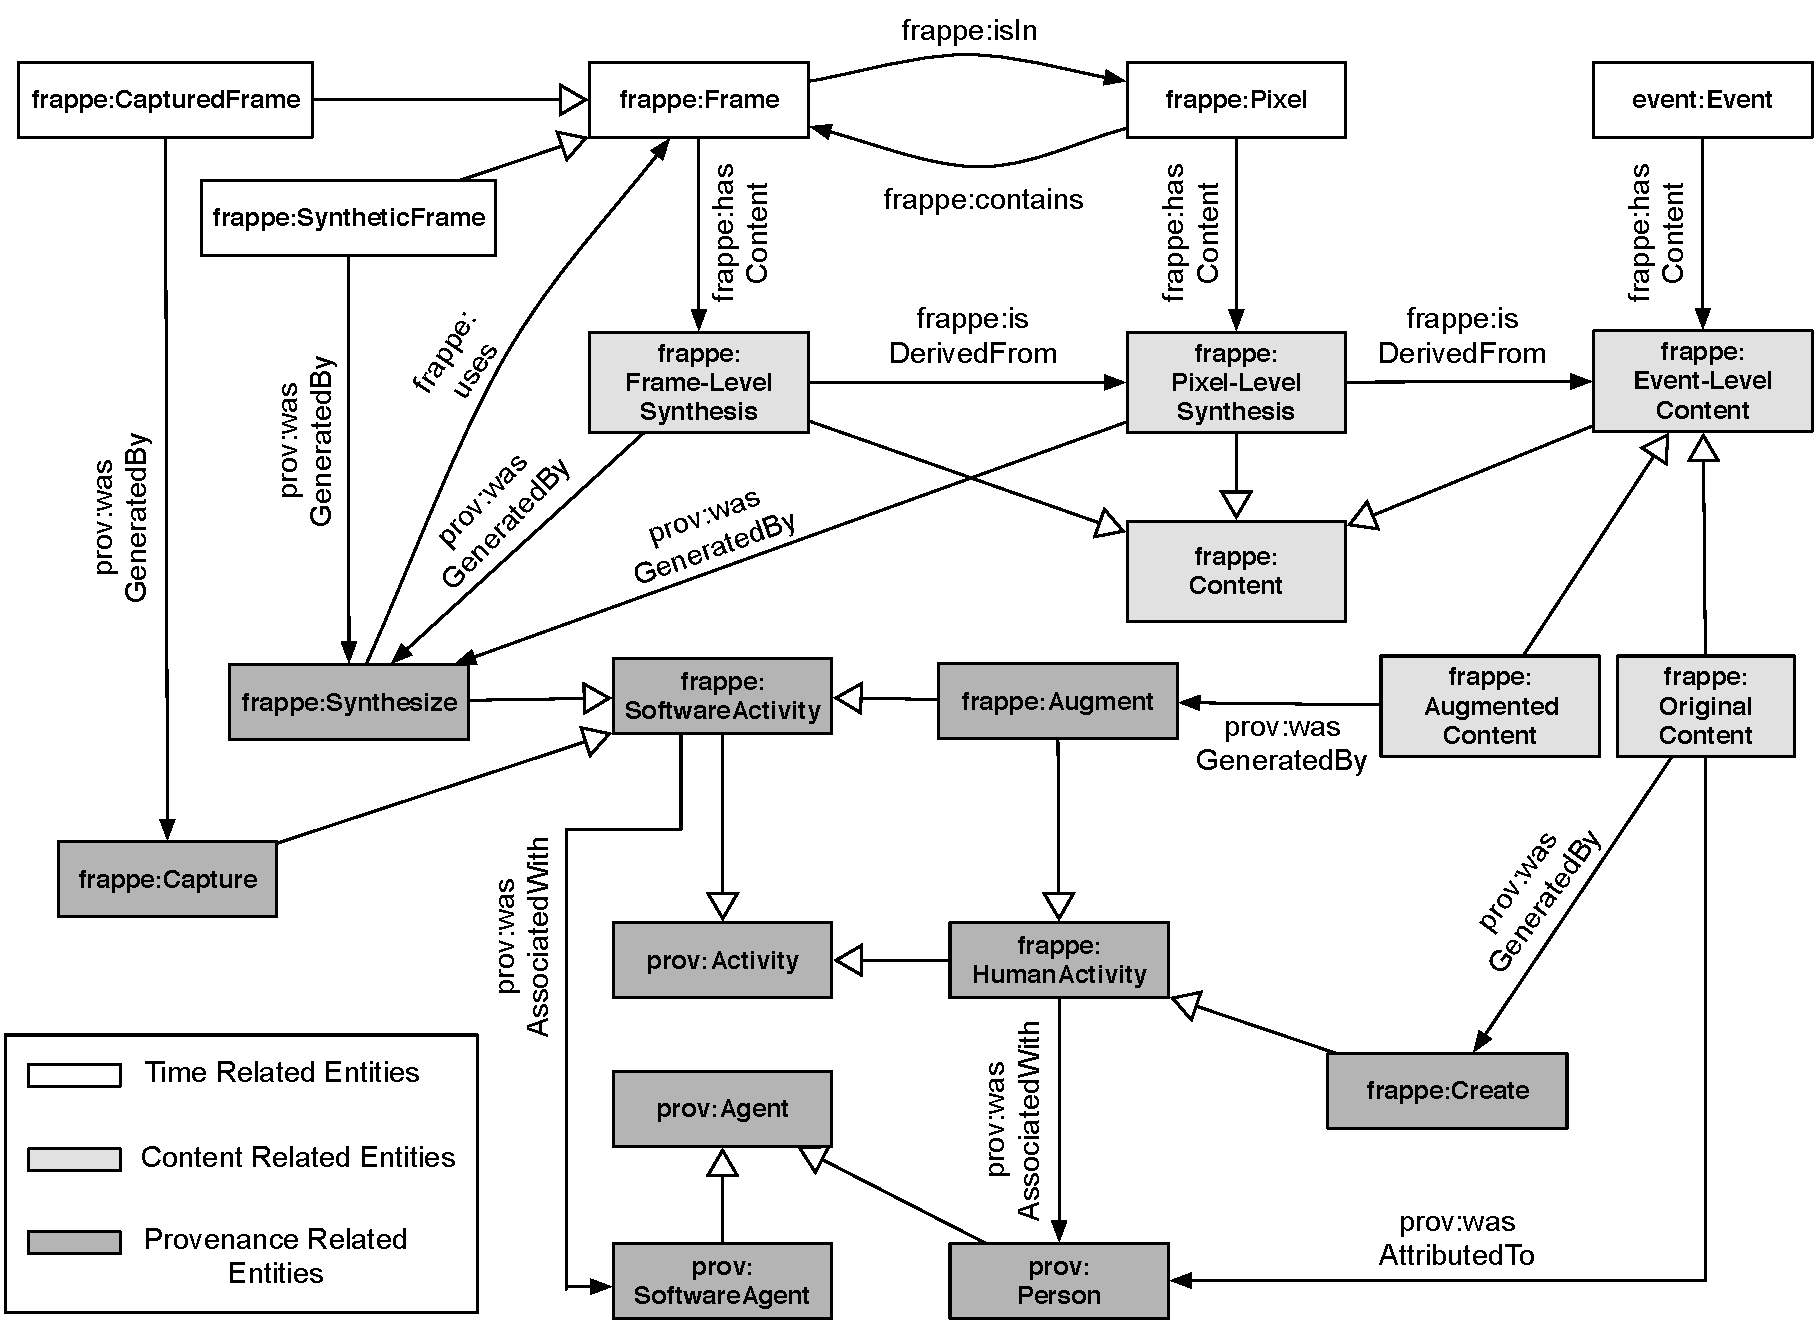
\includegraphics[width=0.95\textwidth]{img/conceptual-model-extended-core}
\caption{The extended version of the \frappe{} model, represented as a colored UML diagram highlighting time-, content-, and provenance- related concepts.}
\label{fig:extended-core}
\end{figure} 

The temporal fragment (the classes \textsf{Frame}, \textsf{Pixel} and \textsf{Event}) and the spatial fragment (the classes \textsf{Grid}, \textsf{Cell} and \textsf{Place}) are inherited from \frappe{} 1.0.
For a detailed description of these parts we refer the reader to Section~\ref{sec:conc-fr-1-mod}

In \frappe{} 2.0, the content can be associated to the time-varying classes and carries information about the event it is associated to.
At event level the content can be \textsf{Original} or \textsf{Augmented}. The original content represents a simple measure or description of a phenomenon, while any enrichment of an original content produces an augmented content.
For instance in a \textit{Tweet} related to the Museum of Modern Art (MOMA),  the \textsf{OriginalContent}, in form of a text, contains different entities presented in different surface forms (e.g., moMA, Museum of Modern Art, etc). The \textsf{Augmentation} allows to link those surface forms to a single db-pedia entity\footnote{\url{http://dbpedia.org/page/Museum_of_Modern_Art}} (see Listing~\ref{lst:sm}).
The content related to \textsf{Pixel} or \textsf{Frame} is \textsf{Synthetic} and it is derived by processing event-related contents. 

In the extended provenance fragment of \frappe{} 2.0, the \textsf{Agent} concept is explicitly defined.
Each activity is performed either by a \textsf{HumanAgent} or by a \textsf{SoftwareAgent}. Consequently, the two \textsf{Agent}s \textsf{wasAssociatedTo}, respectively, \textsf{HumanActivity} or \textsf{SoftwareActivity}. 
On the one hand, an example of \textsf{HumanActivity} is the \textsf{Create} activity, exploited to create an \textsf{OriginalContent}. On the other hand, a \textsf{SoftwareActivity} can be exemplified by the \textsf{Synthesize} activity, used to create a \textsf{Synthetic} content associated to a \textsf{Pixel} or a \textsf{Frame}.

We developed \frappe{} 2.0 keeping in mind the evaluation based on Tom Gruber's principles presented in Section~\ref{sec:conc-fr-1-eval} and it also complies to them.
\frappe{} 2.0 keeps satisfying the \textit{clarity} principles because we add common terms in provenance and content analytics domains. \frappe{} 2.0 remains as general as possible in order to satisfy the \textit{minimal encoding bias} and the \textit{minimal ontological commitment} principles. \frappe{} 2.0 is still \textit{coherent} and the use cases in the Chapter~\ref{ch:case-studies} demonstrates its \textit{extendibility}.

\section{\frappe{} 2.0 and Urban Data Analysis} \label{sec:conc-fr-2-analysis}

In this section, we summarize the methods we use in exploiting \frappe{} to enable the three classic dimensions of the urban data analysis (see Section~\ref{sec:uda-analysis}).
The use cases, presented in Chapter~\ref{ch:case-studies}, offer an overview of the \frappe{} capabilities in enabling all the classic urban data analysis categories.

Concerning the Content Analysis, as mentioned in the Section~\ref{sec:conc-fr-2}, \frappe{} enables the association of the information content to an event, with all the indirect information related to time and space.

\begin{figure}[p]
\begin{minipage}{0.95\linewidth}
\begin{lstlisting}[label={lst:sm}, caption={The \frappe{} representation of a social message}, style=N3]
@prefix frappe:<http://streamreasoning.org/ontologies/frappe#>
@prefix frPlace: <http://streamreasoning.org/frappe/Places/> .
@prefix frEvent: <http://streamreasoning.org/frappe/Events/> .
@prefix frContent: <http://streamreasoning.org/frappe/Content/> .
@prefix frAct: <http://streamreasoning.org/frappe/Activity/> .
@prefix frAgent: <http://streamreasoning.org/frappe/Agent/> .
@prefix frEntity: <http://streamreasoning.org/frappe/Entity/> .
@prefix xsd:<http://www.w3.org/2001/XMLSchema#>
@prefix time:<http://www.w3.org/2006/time#>
@prefix prov:<http://www.w3.org/ns/prov#>
@prefix event:<http://purl.org/NET/c4dm/event.owl#>
@prefix rdfs:<http://www.w3.org/2000/01/rdf-schema#>

frEvent:E a frappe:messageSending ; 
  a event:Event ;
  event:time [ a time:Instant ;
    time:inXSDDateTime "2018-07-10T10:00:00"^^xsd:dateTime ] ;
  frappe:location frPlace:P ;
  frappe:hasContent frContent:oc  ;
  frappe:hasContent frContent:ac  .

frContent:oc a frappe:OriginalContent ;
  frappe:litContent "At Museum of Modern Art to see Claude Monet, Water Lilies #moMA"^^xsd:string ;
  prov:wasGeneratedBy frAct:cActivity ;
  prov:wasAttributedTo frUser:user .

frAct:cActivity a frappe:Create ;
  a frappe:HumanActivity ;
  prov:wasAssociatedWith frAgent:user .
    
frAgent:user a frappe:HumanAgent ;
  a prov:Person .

frContent:oc a frappe:AugmentedContent ;
  frappe:dbPediaEntity frEntity:MOMA ;
  frappe:dbPediaEntity frEntity:Claude_Monet ;
  frappe:dbPediaEntity frEntity:Water_Lilies ;
  prov:wasGeneratedBy frAct:aActivity .

frEntity:MOMA a prov:entity ;
  prov:value ".../Museum_of_Modern_Art"^^xsd:anyURI ;

frEntity:Claude_Monet a prov:entity ;
  prov:value ".../Claude_Monet"^^xsd:anyURI ;

frEntity:Water_Lilies a prov:entity ;
  prov:value ".../Water_Lilies_(Monet_series)"^^xsd:anyURI ;
    
frAct:aActivity a frappe:Augment ;
  a frappe:SoftwareActivity ;
  prov:wasAssociatedWith frAgent:sa .

frAgent:sa a frappe:SoftwareAgent ;
  rdfs:label "DBpediaSpotlight"^^xsd:string;
\end{lstlisting}
\end{minipage}
\end{figure}

Listing~\ref{lst:sm} represents the sending event of a micropost by a social media user.
The listing mainly focuses on the \frappe{} 2.0 extensions (content and provenance).
According to the \frappe{} conceptual model, the \textsf{messageSending} \textsf{Event} is described by a set of properties, including the \textsf{Event-RelatedContent}.
\frappe{} 2.0 distinguishes between two different types of this content, the \textsf{OriginalContent} and the \textsf{AugmentedContent}.
In the example, the \textsf{OriginalContent} is the text of the message and is produced by a \textsf{Create} activity, performed by a \textsf{Person}. Contrariwise, the \textsf{AugmentedContent} is created by the DBpediaSpotlight \textsf{SoftwareAgent} that automatically extract the DBpedia entities from the \textsf{OriginalContent}.

\frappe{} enables the Spatial Analysis mainly through the concepts of \textsf{Grid} and \textsf{Cell}. 
Moreover, thanks to their common sense, the \textsf{Grid} and \textsf{Cell} concepts improve the understandability and navigability of geographical-based content. 
They can be instantiated in multiple ways: we may define different types of grids and cells, based on the specific data sets and on the analysis needs. We identify three main categories of grids: 

\begin{itemize}
\item \textit{Regular squared grid}:  a regular \textsf{Grid} dividing the physical space in cells that are uniform for shape, size, and positioning. For instance, in many of our experiences around the city of Milan (see Section~\ref{sec:cs-mdw}), we defined a \textsf{Grid} of 100 x 100 \textsf{Cell}s, each \textsf{Cell} having a size of 250 x 250 meters.

\item \textit{Irregular grid with official business-driven meaning}: a \textsf{Grid} of \textsf{Cell}s that are different in shape, size and orientation based on some official definition (e.g., the boroughs or zones of a city) or based on some business specification (e.g., the commercial areas of the city). An example of this can be the official city districts defined by the municipality or the areas where a large \textsf{Event} is located. During our experiences in Milan we used the definitions of the official MDW areas to perform aggregated analysis on the data (see Section~\ref{sec:cs-mdw}).

\item \textit{Irregular grid with data-driven definition}: a \textsf{Grid} of \textsf{Cell}s defined bottom-up based on the domain data available or on partial analysis and aggregations already performed on them. Some examples include the areas served by different electricity sub-stations, the mobile phone cell coverage, or the areas where mobile phone presence can be clustered with sufficient precision with respect to the location of the antennas. During our work in Como (see Section~\ref{sec:cs-como}), we experienced data-driven definition of different areas related to the mobile network coverage. 

\end{itemize}
Another important feature of the \textsf{Grid} is the coverage of the area of interests. We can define \textsf{Grid}s with \textbf{total coverage} or \textbf{partial coverage}. Typically, regular \textsf{Grid}s tend to feature total coverage, while irregular ones, especially when defined starting from business requirements, may offer only a partial coverage of the area.

All the relevant spatial analysis exposed in Section~\ref{sec:uda-analysis} (i.e., Dispersion, Distance and relation to places, Correlation and Prediction) can be performed exploiting the concept of \textsf{Grid} and \textsf{Cell}.

The Temporal analysis in \frappe{} can be described as the study of the evolution and spreading of signals captured by \textsf{Pixel}s, which refers to \textsf{Cell}s, over time in different \textsf{Frame}s.
\frappe{} enables all the categories of the temporal analysis described in Section~\ref{sec:uda-analysis}.
The \textsf{Description} in \frappe{} describe the signal \textsf{captured} by \textsf{Pixel}-level contents to create a time-series. \frappe{} enables the \textsf{Correlation}, \textsf{Prediction}, \textsf{Anomaly detection} and \textsf{Causality} analysis exploiting the concepts of \textsf{Pixel} and \textsf{Frame}. 

Finally, \frappe{} exploits the links between \textsf{Cell} and \textsf{Pixel}, \textsf{Grid} and \textsf{Frame} to enable the combination of time and space analysis. 

\section{Conclusion}
In this chapter, we study the problem of modeling spatio-temporal data to enable analyses that involve time, space and content aspects of the data. 
The growing availability of geo-located time-varying data, in particular in the urban environment, increased the needs for an holistic conceptual model to describe the data itself, its dynamics and to enable advanced analysis.

To address this problem, we proposed \frappe{} conceptual model. 
\frappe{} exploits digital image processing terms to tame three main dimensions of analysis: space, time, and content.
It uses image processing common terms to create a bridge between the data engineers and visual interface designers and enables visual analytics on geo-spatial time varying data.

We first developed \frappe{} 1.0 using state of the art methodology (METHONTOLOGY).
It is formalized using OWL2 and reuses already existing ontologies (see Section~\ref{sec:conc-fr-1-mod} for further details).
We then extended \frappe{} to version 2.0 by adding concepts related to the provenance and the content (see Section~\ref{sec:conc-fr-2} for additional details on the extension).

In order to validate Hypothesis \textsf{Hp.1.1}, we checked the adherence of \frappe{} 1.0 to the five Tom Gruber's principles (see Section~\ref{sec:conc-fr-1-eval}).
The \textit{clarity}, \textit{minimal encoding bias} and \textit{coherence} is respected by construction. 
Infact, the \frappe{} 1.0 definitions are documented in natural language, they are formalized using OWL2 standard and all the inferred data is meaningful and consistent.  
Moreover, \frappe{} 1.0 requires a \textit{minimal ontological commitment} because it easily allows specialization, while its \textit{extendibility} is ensured by the number of use cases that are based on it.

Our extended usage of \frappe{} 1.0 in real world use cases (see Chapter~\ref{ch:case-studies}) pushed us to create \frappe{} 2.0 that contains the formalization of the concepts that we used more often in our use cases.
They are related to the provenance of the information and to the content of the events.
Also \frappe{} 2.0 results \textit{clear}, \textit{coherent}, \textit{extendable} and with \textit{minimal encoding bias}.
Moreover, it still requires a \textit{minimal ontological commitment}, since the new concepts has been formalized because they are shared by two or more use cases.

The overall evaluation, based on Tom Gruber's Principles, validates the Hypothesis \textsf{Hp.1.1}.
The presentation of the validation of the Hypothesis \textsf{Hp.1.2} is postponed to Chapter~\ref{ch:case-studies} because it is based on the empirical evaluation of the guessability of the use cases' visualizations.